\documentclass[12pt, twoside, openany]{report}
\usepackage[dvips]{graphicx,color,rotating}
\usepackage{a4wide}
\usepackage[utf8]{inputenc}
\usepackage{enumerate}
\usepackage{verbatim}
\usepackage[polish,british]{babel}
\usepackage[T1]{fontenc}
\usepackage{geometry}
\geometry{left=25mm,right=25mm,%
bindingoffset=10mm, top=25mm, bottom=25mm}
\usepackage{latexsym}
\usepackage{amsthm}
\usepackage{palatino}
\usepackage{array}
\usepackage{pstricks}
\usepackage{textcomp}
\theoremstyle{definition}
\newcommand*{\norm}[1]{\left\Vert{#1}\right\Vert}
\newcommand*{\abs}[1]{\left\vert{#1}\right\vert}
\newcommand*{\om}{\omega}

\author{Paweł Paczuski}
\title{Tytuł pracy}

\begin{document}

% Zażółć gęślą jaźń.
\begin{titlepage}
\pagestyle{empty}

\noindent
\begin{Large}
\begin{table}[t]
\centering
\begin{tabular}[t]{lcr}
 
\includegraphics[width=70pt,height=70pt]{PW} & POLITECHNIKA WARSZAWSKA & \includegraphics[width=70pt,height=70pt]{ELKA}\\
& WYDZIAŁ ELEKTRONIKI & \\
& I TECHNIK INFORMACYJNYCH &
\end{tabular}
\end{table}

% \vfill
\begin{center}ENGINEER DIPLOMA THESIS\end{center}
\begin{center}Computer Science\end{center}\end{Large}
% \vfill
\begin{center}
\Huge
\textbf{Structured reporting system}
\end{center}
% \vfill\vfill
\vfill
\begin{center}
\Large
Author:\\
\LARGE
Paweł Paczuski
\end{center}
\vfill
\begin{center}
\Large
Thesis supervisor: prof. dr hab. inż. Jan J. Mulawka
\end{center}
\vfill
\begin{center}
\Large
Warsaw, June 2018
\end{center}
\newpage
\hfill
\begin{table}[b]
\centering
\begin{tabular}[t]{ccc}
............................................. & \hspace*{100pt} & .............................................\\
podpis promotora & \hspace*{100pt} & podpis autora
\end{tabular}
\end{table}


% \maketitle
\end{titlepage}
\thispagestyle{empty}
\newpage
\pagestyle{headings}
\setcounter{page}{1}
\hyphenation{Syl-ves-tra}
\hyphenation{Syl-ves-ter-a}
\begin{otherlanguage}{british}
\begin{abstract}
Structured radiological reporting system.

Design and implementation of a system that can be used by radiologists to create structured radiological reports. The system uses sets of standardized, frequently used phrases to: describe state of patient's body captured by other medical diagnostics methods, provide set of tools that minimize risk of mistake and increase productivity. 
\end{abstract}
\end{otherlanguage}

\begin{otherlanguage}{polish}
\begin{abstract}
streszczenie po polsku
\end{abstract}
\end{otherlanguage}

%-----------Początek części zasadniczej-----------

\chapter{Introduction}
\section{The need for medical diagnostics}
Everyday millions of physicians treat injuries and illnesses. Before a doctor can plan an individual treatment for a patient, they have to diagnose which organs are in pathological states\cite{bls}. This sometimes can be achieved by simply glancing at the body, however, there are many illnesses that require specialized set of tools and methods in order to observe which parts of patient's body are in an unwanted state. Through years of research, many different techniques were established and a separate specialization emerged -- radiology. Radiologists focus mainly on analyzing and interpreting diagnostic imagery and as a result of their work they create a document called radiological report which contains description of what can be observed in the image of patient body. Reports may contain description of state of particular organs, measurements (eg. radius, volume, concentration of certain substances in the blood), comparison of medical condition of a patient observed at different times and description of overall state of the patient. \\
\section{Existing solutions}
Currently, the research is focused on finding new ways of diagnosing diseases by  the use of more advanced equipment or brilliant algorithms that try to automate image analysis \cite{ai}. \\
On the other hand, there exist initiatives that try to improve quality of the radiological reports themselves. There are groups consisting of both computer scientists and physicians that try to standardize reports, prepare checklists that require doctors to describe patients' state in particular order and create a set of phrases that will be understood in the same way by all physicians \cite{snomed}. A lot of work has been done to provide common medical nomenclature for medical conditions, provide theoretical framework to describe relations between causes and effects of patients' condition. As there are more and more methods used to diagnose, the amount of information captured increases, so the reporting methodology has to be kept up to date with the state of art. This is why a very specific field -- structural reporting (SR) emerged. The basic idea is to provide a way to create radiological reports that convey as much semantics as possible in an easy to follow way. One can find great ideas implemented in such standards as SNOMED SR \cite{sr} and also HL7 version 3 Clinical Document Architecture (HL7 V3 CDA). By using these standards one can encode relations between organs and diseases (causality) in a very regular format. After encoding structure in the report, one can use algorithms to e.g. highlight what changed since last visit, look for diseases that were are diagnosed in the specified time range etc. This is very difficult to achieve when reports are stored in plain text. Structural reporting focuses on encoding only meaning -- the visual representation of resulting reports is a separate matter to discuss \cite{sr}.
In spite of the existence of these standards, it is almost impossible to find software that implements structural reporting techniques. One of the most important reasons is the fact that in order to understand benefits of SR, one has to acquire certain level of understanding of the typical workflow of a radiologist. 
\\ \\
\section{Definition of the engineering problem}
In this thesis I present a solution to the problem of not satisfactory productivity of radiologists by implementing a program used to create structured radiological reports. The system uses sets of standardized, frequently used phrases to: describe state of patient's body captured by other medical diagnostics methods, provide set of tools that minimize risk of mistake and allows radiologists to create reports faster.

\section{Typical workflow of a radiologist in Poland}
In order to find places where optimization of productivity could be applied, one has to get to know how a radiologist works and what are activities that waste significant amounts of time. \\
In a medium sized clinic, medical imagery is captured by a radiologic technologist who then uploads the data to the radiological information system (RIS) and attaches identification information to the images. This system distributes imagery to the team of radiologists that work for this clinic. 

Imagery can be distributed in one of the following manners:
\begin{itemize}
    \item particular patient is always serviced by the same radiologist or the RIS system 
    \item RIS system acts as an accumulator of images and radiologist decide which patient they focus on next
    \item certain types of medical examinations are are always assigned to a radiologist that is specialized in describing them
\end{itemize}

After receiving diagnostic imagery, a radiologist uses special software called viewer\cite{viewer} to navigate through images, make measurements by using visual tools like virtual ruler and examine what is the state of patient's body. In parallel to this, the doctor uses text editor and describes what he or she sees in the images. 
\begin{figure}
    \centering
    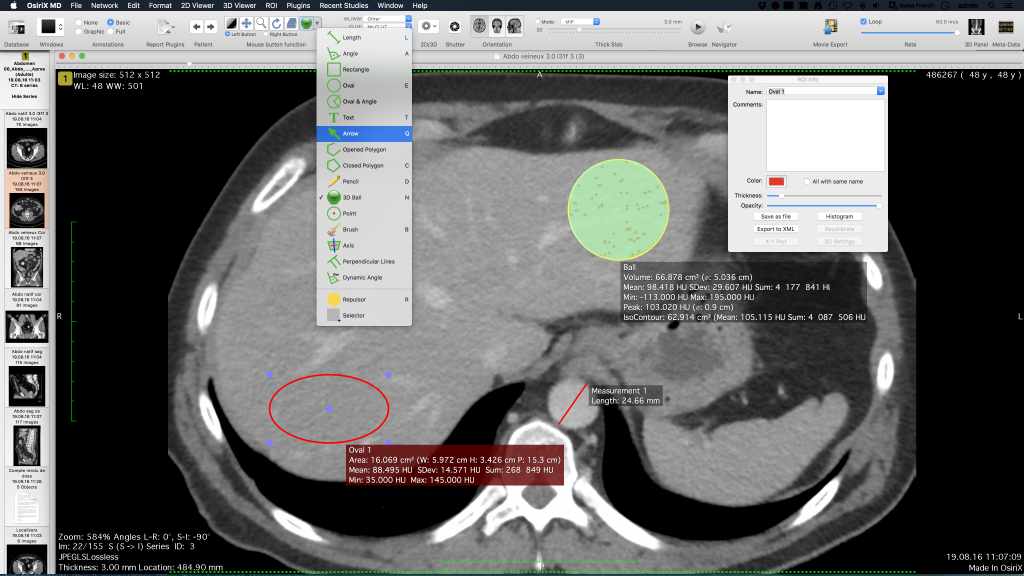
\includegraphics[width=0.9\linewidth]{osirix}
    \caption{OsiriX is one of the most popular image viewers used by the radiologists}
    \label{fig:osirix}
\end{figure}



\section{Discussion about presented workflow}
\subsection{The good parts}
\subsubsection{Viewer software provides expected functionality}
Viewer software has a very stable position on the market and is perfectly tailored to the needs of a radiologist. It often uses advanced techniques of 3D graphics to present patient's body as accurately as possible.
\subsubsection{RIS systems make it easy to exchange data between physians}
There is no need need for the radiologist to deliver the radiological report to the other physician personally as it is done automatically. Also, RIS systems provide good means of distributing diagnostic imagery to radiologists.
\subsection{The bad parts}
\subsubsection{Focus on text rather than semantics}
It is expected that the radiologist will produce a consistent, ordered report by means of text editors. Some RIS systems provide basic text formatting functionality like italicization, underlining but they are very limited to the textual presentation of the report. There are no means to encode relations in this representation.
\subsubsection{Each radiologist has their own style of writing}
Usually there are no structural expectations about the resulting report. Each radiologist can have their own style of writing, order of organs and observation. This leads to the waste of time as people who read the report have to make some effort to infer the meaning. 
\subsubsection{Selective description}
It is very frequent that radiologists include in the report only things that they consider bad for the patient. This makes the report more goal-oriented but it means that it is useless to get to know the overall state of patient body.
\subsubsection{Copy-paste}
Radiologists try to solve the problem of typing on their own by crating templates that contain certain pathologies listed and all they do is the commonly called 'copy-paste' method to create report content. Sometimes they do not notice parts of copied text that are different from the actual state of the body so the reports may contain observations that are false. 

\section{Other ways to create radiological reports}
In many English-speaking countries the workflow of a radiologists differs in the way the radiological report is generated. The radiologists records their voice while examining the imagery. The recordings are then transcribed using either speech recognition algorithms or manually by technologists
\section{Thesis scope and objectives}
\section{Description of contents}
\chapter{Short review of types of software used in healthcare}
\chapter{Description of the proposed solution}
\chapter{Implementation }
\chapter{Examples of application}

\chapter{Conclusion}
\appendix {How to use the program}


%-----------Koniec części zasadniczej-----------

\begin{thebibliography}{11}
\bibitem{bls} https://www.bls.gov/ooh/healthcare/physicians-and-surgeons.htm, accessed 08.10.2017 13:30
\bibitem{ai} M. Recht, N. Bryan, Artificial Intelligence: Threat or Boon to Radiologists?

N1  - doi: 10.1016/j.jacr.2017.07.007
\bibitem{snomed} T. Benson, Principles of health interoperability HL7 and SNOMED.
\bibitem{sr} D. A. Clunie, DICOM Structured Reporting
\bibitem{hl7cda} http://www.hl7.org/Special/committees/structure/index.cfm 
\bibitem{techonologist} https://www.asrt.org/main/careers/careers-in-radiologic-technology/who-are-radiologic-technologists
\bibitem{workflow} https://radiologystories.com/2013/10/31/the-typical-radiologist-work-day/
\bibitem{viewer}
http://www.osirix-viewer.com/osirix/overview/
\bibitem{speech-impact}
S. Langer, Impact of Speech Recognition on Radiologist Productivity

\bibitem{speech-africa} J. du Toit, R. Hattingh and R. Pitcher, The accuracy of radiology speech recognition
reports in a multilingual South African teaching hospital.
\end{thebibliography}
\tableofcontents
\clearpage
\begin{otherlanguage}{polish}
\pagestyle{empty}
\noindent Warszawa, dnia ...............
\vspace{5cm}
\begin{center}
\LARGE{Oświadczenie}
\end{center}
Oświadczam, że pracę inżynierską pod tytułem: ,,Tytuł pracy'', której promotorem jest prof. dr hab. Jan Wybitny, wykonałem/am samodzielnie, co poświadczam własnoręcznym podpisem.
\vspace{2cm}
\begin{flushright}
...........................................
\end{flushright}
\end{otherlanguage}
\end{document}